\subsubsection{Exercise}

Now that our controller fulfill the criteria about the disturbance attenuation we need to improve it by accelerating the system and controlling the overshoot. 

\paragraph{Lead-controller design}

To do so we add a lead-controller to $F_y$: $F_{lead} = K \frac{\tau_D s + 1}{\beta \tau_D s +1}$.
Using the same method as the one depicted in Exercise \ref{exo411}, we have the following values for the parameters:
\begin{shortitemize}
    \item $K = 1.35$
    \item $\beta = 0.76$
    \item $\tau_D = 0.078$
\end{shortitemize}

We meet the following specifications:

\begin{center}
\begin{tabular}{|c|c|}
    \hline
    Phase margin & $15^{\circ}$ at $\omega_C = 15$ rad/s \\ 
    \hline
    Rise time $t_r$ & $0.07$s\\
    \hline
    Overshoot $D\%$ & $24\%$ \\ 
    \hline
\end{tabular}
\end{center}

The overshoot is still bigger than the $10\%$ required. 

Figure \ref{designLeadLag} shows the step response of the system and the response to a step in the perturbation. 

\begin{figure}[h!t]
    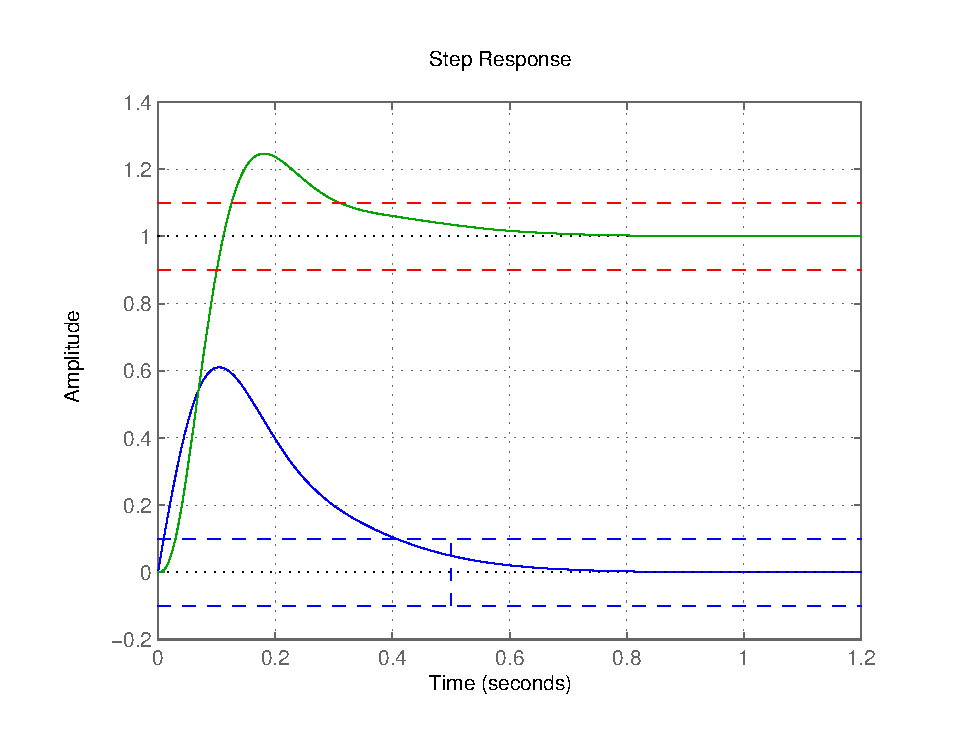
\includegraphics[width=\columnwidth]{fig/designLeadLag.eps}
    \caption{Step response of the system (green) and response to a step in the disturbance (blue) with the addition of the lead-controller}
    \label{designLeadLag}
\end{figure}

Now that we have added the lead-controller, the expression of $F_y$ is the following:

$$F_y = K \frac{\tau_D s + 1}{\beta \tau_D s +1}\frac{s + \omega_I}{s} \frac{\omega_0\omega_1}{(s+\omega_0)(s+\omega_1)} G^{-1} G_d $$


\paragraph{Prefilter design}

Once this lead-controller is added to the feedback controller we want to create a prefilter $F_r$ to fulfill all specifications. 

Let:

$$F_r = \frac{1}{1 + \tau s}$$

The value of $\tau$ is tuned in order to get $|u(t) < 1$ for all $t$.

With $\tau = 0.14$, \textbf{all the criteria are met} and $\max_{t} |u(t)| = 0.98$.

Figure \ref{designFr} shows the step response of the system and the response to a step in the perturbation.



